% !TeX spellcheck = en_US
\documentclass[c,8pt,xcolor...,x11names,handout ]{beamer} % ,handout
\usepackage{icclslides}
\usepackage[latin1]{inputenc}
\usepackage[british]{babel}
\usepackage{amssymb}
\usepackage{latexsym}
\usepackage{rotate}
\usepackage{tikz}
\usepackage{verbatim}
\usepackage{colortbl}
\usepackage{booktabs}
\usepackage{ulem}
% \usepackage{arydshln}
%\usepackage{pdfpages}hord
\usepackage{graphicx} 
\usepackage{tikzsymbols}
\usepackage{tikz}
\usepackage{subcaption}
\usepackage[export]{adjustbox}
\usepackage{pdfpages}
\usetikzlibrary{positioning}

\tikzstyle{ele} = [circle, text centered, minimum width=1em, minimum height=3ex]

%% Uncomment to activate navigation symbols in the lower right of the pages:
\setbeamertemplate{navigation symbols}{}
%\setbeamercovered{transparent}

\renewcommand{\Myauthor}{Martin R\"obke}
\renewcommand{\Mytitle}{Visualizing Dynamic Programming On Tree Decompositions}
\usepackage{showexpl} 

\lstloadlanguages{[LaTeX]Tex} 
\lstset{% 
     basicstyle=\ttfamily\small, 
     commentstyle=\itshape\ttfamily\small, 
     showspaces=false, 
     showstringspaces=false, 
     breaklines=true, 
     breakautoindent=true, 
     captionpos=t 
} 

\begin{document}
\begin{frame}
%	Frequently asked questions during the defense of the bachelor thesis:
%What motivated you to write your Bachelor's thesis on exactly this topic?
%They often use the term X. Can you explain it in more detail?
%We miss the point Y in your work. What can you say to this?
%For what reason did you decide on the methodology you use?
%What added value has your research delivered?
%To what extent is your research relevant?
	\customtitle
	\begin{center}
		\begin{minipage}{0.5\textwidth}
			\begin{itemize}
				\item {\sc What} is the motivation
				\item {\sc Who} benefits from visualization?
				\item {\sc Challenges}  and solutions
				\item {\sc What} could be used otherwise?
				\item {\sc Outlook} and ideas
			\end{itemize}
		\end{minipage}
	\end{center}

\end{frame}

%%%%%%%%%%%%%%%%%
\section{The task} 


%\begin{frame}
%	\frametitle{Task definition}
%\textit{Investigate how to automatically visualize dynamic programming algorithms based on existing implementations. Integrate your tool into at least one existing implementation, explain details on your implementation, how the visualization works, and show how this can be used for debugging algorithms.}
%
%%The algorithms exploit structural properties in the given problem instance and solve the problem faster if for example the treewidth of a graph representation is small, since they usually run exponentially in the treewidth and polynomially in the size of the input instance. In fact, recent research showed that implementations of dynamic programming algorithms can also compete with modern solvers and even outperform them in projected model counting.
%%Unfortunately, those algorithms are fairly hard to implement. While recent approaches have also investigated on allowing for easier implementations of dynamic programming algorithms on tree decompositions, implementations are still incredibly error prone, in particular, since they often involve bit fiddling and low level operations to make them run efficiently. Investigate how to automatically visualize dynamic programming algorithms based on existing implementations. Integrate your tool into at least one existing implementation, explain details on your implementation, how the visualization works, and show how this can be used for debugging algorithms.
%\medskip
%
%
%\end{frame}

%%%%%%%%%%%%%%%%%%%%%%
\section{Motivation}

\begin{frame}
	\frametitle{Motivation}
	
	\begin{itemize}
		\item DP-on-TD-algorithms can solve Model Counting and various combinatorial problems and are provable efficient at it
		\item Implementations of those are competing with modern solvers
		\bigskip
		\item {\Large But: those are fairly tedious to implement efficiently}
%		as they involve bit fiddling
% it is extremely space intensive (and much more than SAT solving or similar; and you don't really work with compact representations)
		\bigskip
		\item Often bugs in the implementation
		\item Model counting is extremely space intensive (much more than SAT)
%		Practical program information quickly becomes very large (GB)
		
	\end{itemize}
\medskip
%		The B.T. probably focused too much on the convenience features, and not on the urgent need for better debugging and visualization needs for those algorithms.

%Recent research showed that implementations of dynamic programming algorithms can also compete with modern solvers. \\
%Unfortunately, those algorithms are fairly hard to implement  to make them run efficiently.
%
%=> Debug output wird schnell un�bersichtlich/gro�
%Ursprung von Problemen auffinden => (MinVC) Beispiel
\end{frame}

%%%%%%%%%%%%%%%%%%%%%%
\section{Contribution}

\begin{frame}
	\frametitle{Contribution}
This thesis created tdvisu as a tool that 
\medskip
\begin{itemize}
	\item integrates into existing implementations
	\item statically exports data from runs
	\item compiles simple DOT files and SVG graphics
\end{itemize}
\bigskip		

For further research it provides
\medskip
\begin{itemize}
	\item starting point for more complex investigations of 
	\begin{itemize}
		\item bug spotting
		\item and fixing by using visualizations
	\end{itemize} 
	
\end{itemize}
	
\end{frame}


%%%%%%%%%%%%%%%%%%%%%%%
%\section{Who should use this}
%\begin{frame}
%	\frametitle{Creating Visualization for:}
%	\begin{minipage}{0.44\textwidth}
%		\emph{Improving}
%		\begin{itemize}
%			\item examples for students
%			\item debugging and improving interaction of complex data-structures
%			\item hotspots
%		\end{itemize}\medskip
%		
%	\end{minipage}
%	\begin{minipage}{0.55\textwidth}
%		\begin{figure}
%			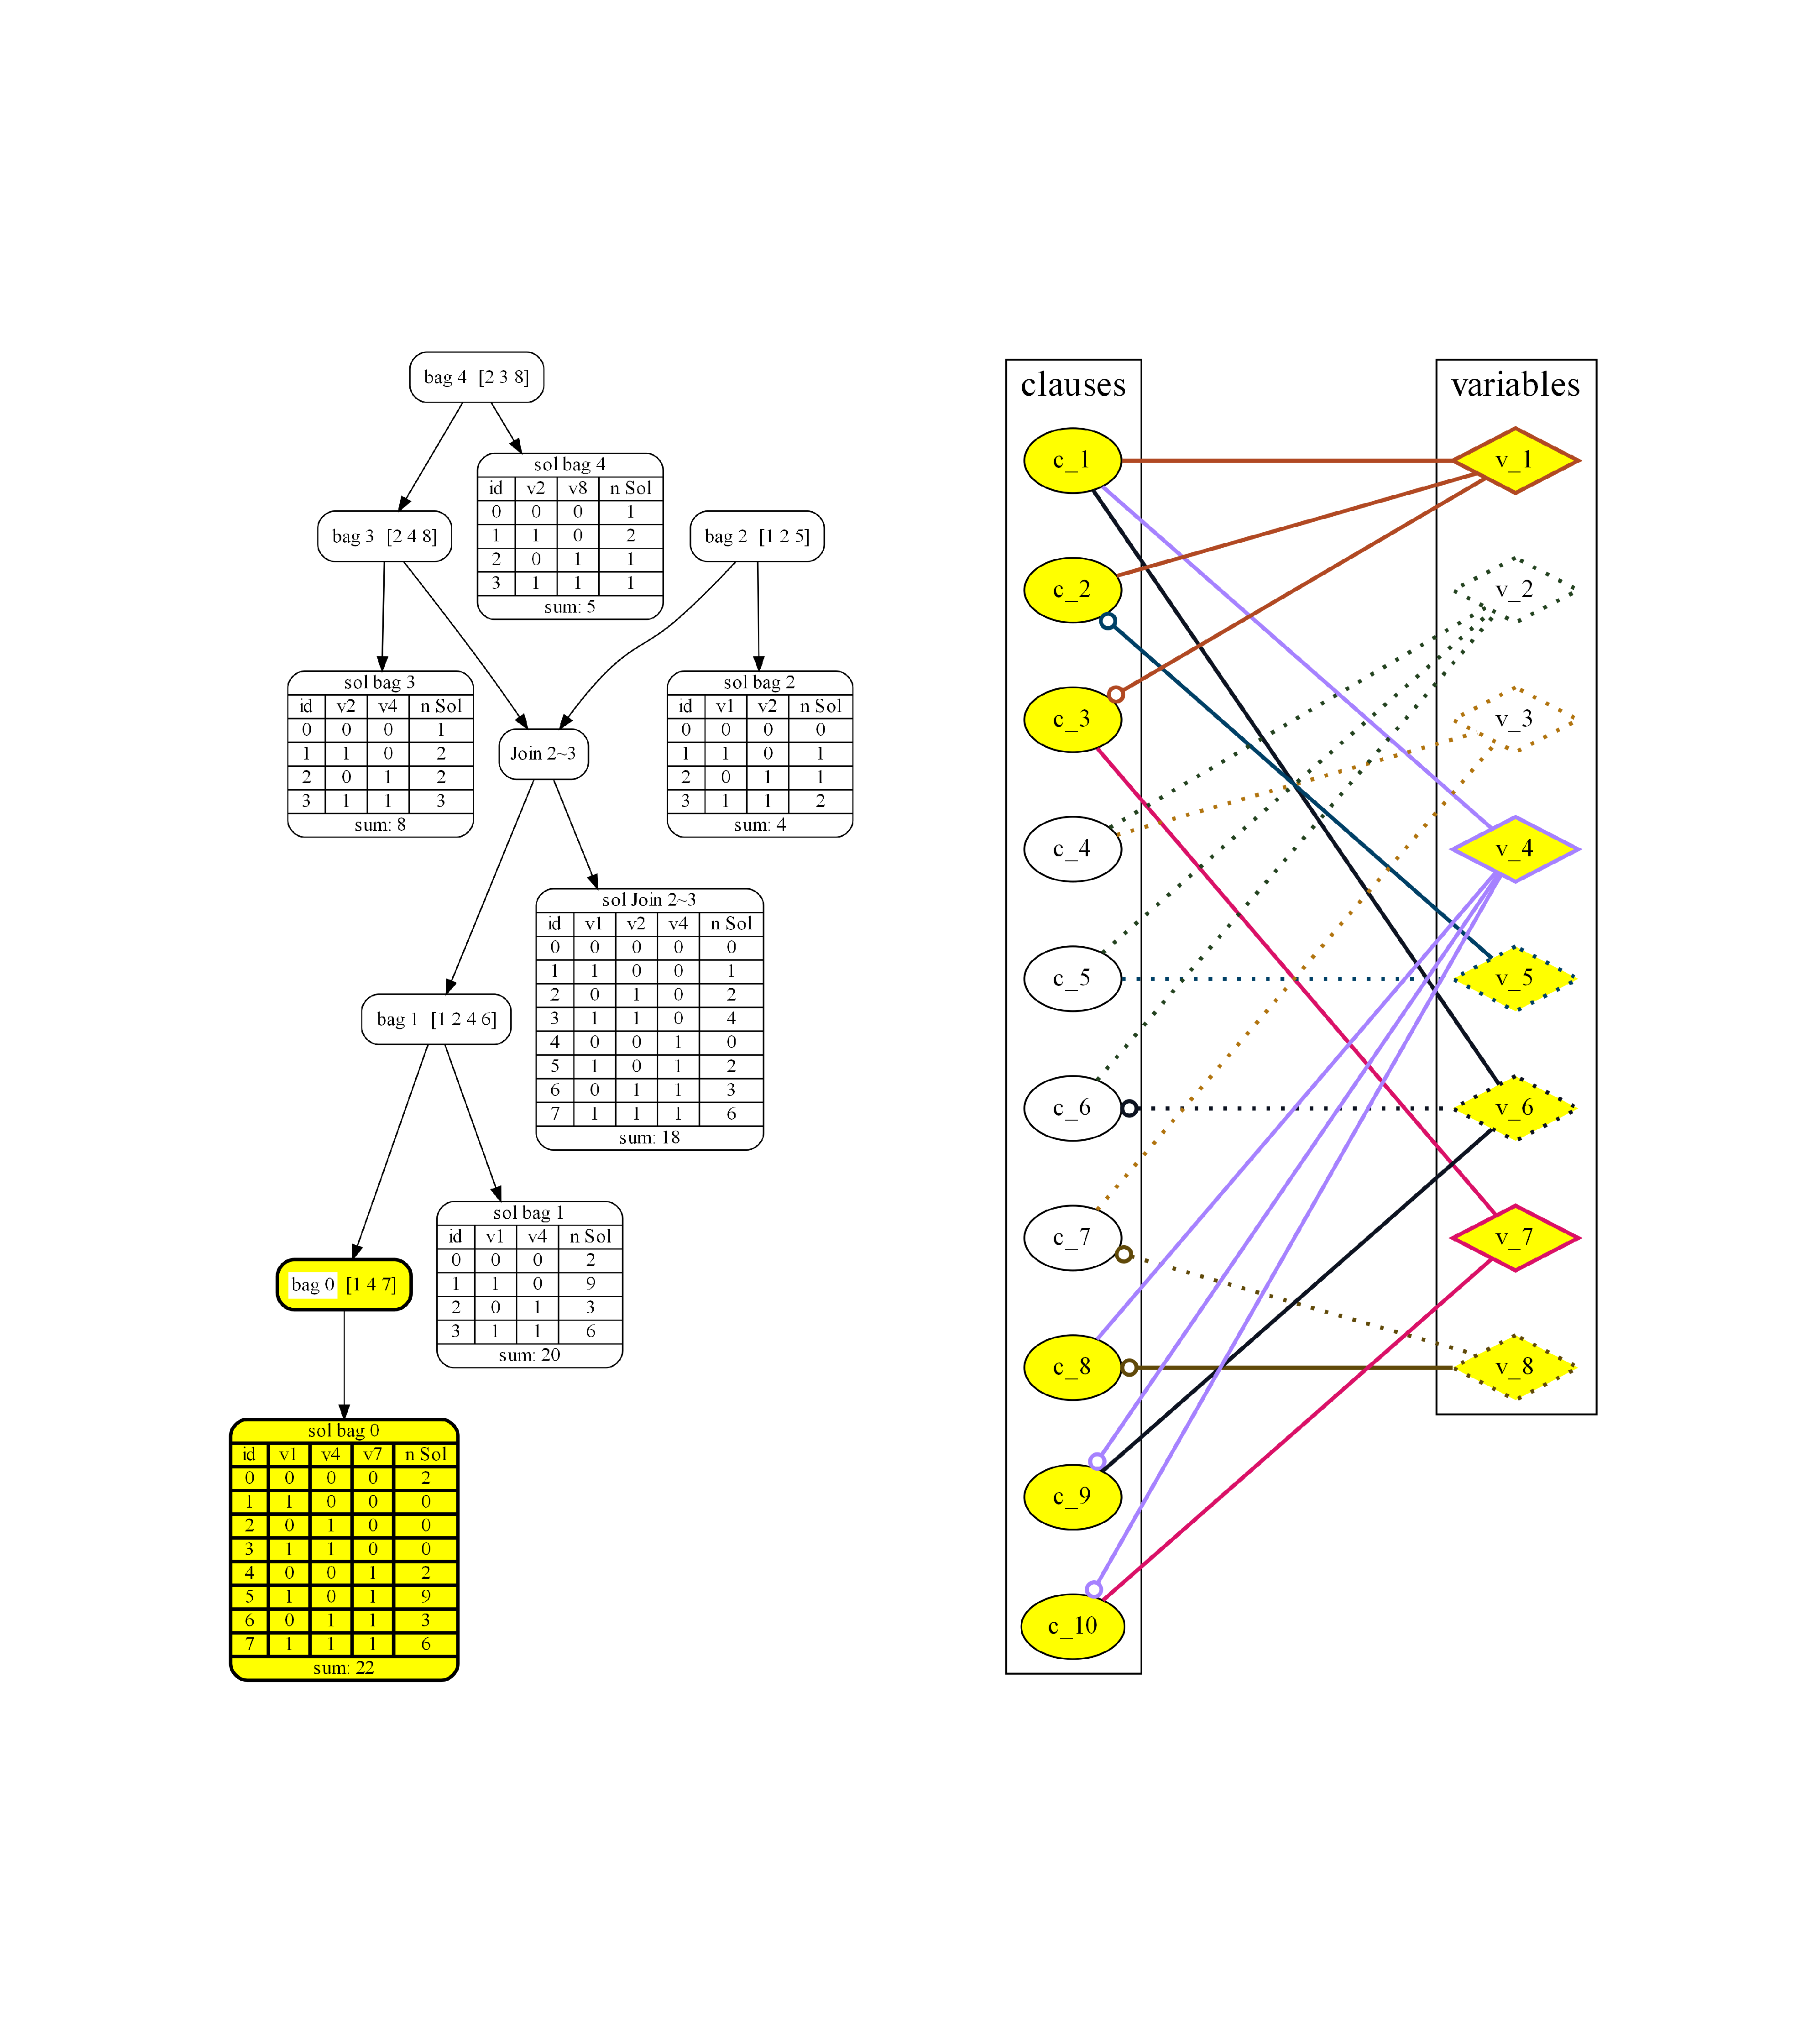
\includegraphics[width=\linewidth]{images/combined8.png}
%		\end{figure}
%	\end{minipage}
%	
%\end{frame}

%%%%%%%%%%%%%%%%%%%%%
\section{Background}
\begin{frame}
	\frametitle{Background}
	\vfill
	The algorithms of interest solve problems of:
	\medskip
	\begin{itemize}
		\item combinatorics (NP-problems)
%		https://de.wikipedia.org/wiki/Karps_21_NP-vollst%C3%A4ndige_Probleme#Liste_der_Probleme
		\item model-counting (\#P-problems)
	\end{itemize}
%	The developed algorithms exist to solve problems of combinatorics (NP-problems) and even the much more work-intensive model-counting (\#P-problems)
%	One consequence of Toda's theorem is that a polynomial-time machine with a #P oracle (P#P) can solve all problems in PH, the entire polynomial hierarchy. In fact, the polynomial-time machine only needs to make one #P query to solve any problem in PH. This is an indication of the extreme difficulty of solving #P-complete problems exactly. 
\bigskip
%=> Kombinatorische Prob. (l�sbare \#P Klasse schwerer(teilweise deutlich komplexer => Referenz Projected Model Counting Markus (hybride Erw dpdb) )) - Algos

%Recent promising results for Projected Model Counting by Markus Hecher\footnote{Hecher M., Thier P., Woltran S. (2020) Taming High Treewidth with Abstraction, Nested Dynamic Programming, and Database Technology. In: Pulina L., Seidl M. (eds) Theory and Applications of Satisfiability Testing - SAT 2020. SAT 2020. Lecture Notes in Computer Science, vol 12178. Springer, Cham. https://doi.org/10.1007/978-3-030-51825-7\_25}.

%We present nested DP, where different levels of abstractions are used to (recursively) compute TDs of a given instance. Further, we integrate the concept of hybrid solving, where subproblems hidden by the abstraction are solved by classical search-based solvers, which leads to an interleaving of parameterized and classical solving. 

Modelcounting: Instead of \textbf{one} solution we want to count \textbf{all} solutions.
\medskip
\begin{figure}
	\centering
	\includegraphics<2>[width=0.7\linewidth]{images/minvcgraph13}
	\includegraphics<3>[width=0.7\linewidth]{images/minvcgraph7.png}
	\label{fig:minvcgraph13}
\end{figure}

\end{frame}

\subsection[TD]{Tree decomposition}
\begin{frame}
	
	\frametitle{Tree Decomposition}
	
	Gives the DP algorithm a partial ordering for sub-problems.
	
%	A tree decomposition is a tree obtained from an arbitrary graph
%	s.t. 
\medskip 
	\begin{enumerate}
		\item \emph{Each vertex} must occur in some
		bag
		\pause
		\item For \emph{each edge}, there is a bag
		containing both endpoints
		\pause
		\item %\emph{Connectedness condition}:\\
		Subgraph ``restricted'' to any vertex must be \emph{connected}
	\end{enumerate}
\pause
	\begin{figure}
		\centering
		\label{fig:tdwheelgraph7}
		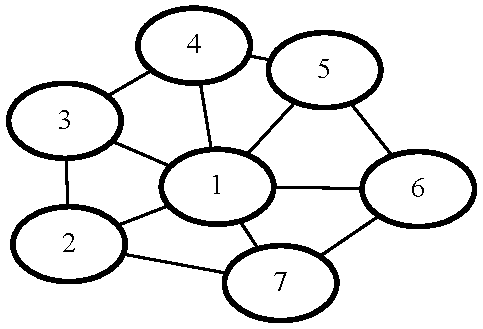
\includegraphics[width=0.38\linewidth]{images/wheelgraph}\quad
		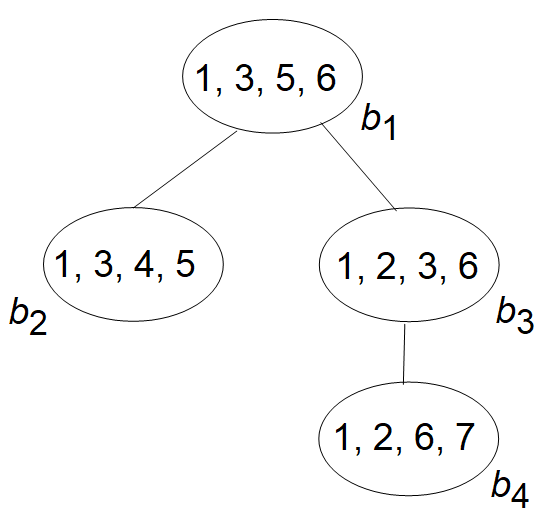
\includegraphics[width=0.38\linewidth]{images/TDWheelgraph7}	
	\end{figure}

\hfill
Width of a TD is: size of largest bag -1\\
\hfill $width = 3$
	
\end{frame}
%{
%	\setbeamercolor{background canvas}{bg=}
%	\includepdf[pages=162-174]{"images/Lecture_pcgp_Summer_2019.pdf"}
%}

%%
\subsection{Instances}
%\begin{frame}
%	\frametitle{(Weighted) Model-Counting}
%\end{frame}

\begin{frame}
	\frametitle{Graphs for Boolean Formulas}
	\smallskip
	\begin{itemize}
		\item {\color{blue} Example set of CNF-clauses:}\smallskip\\
		{\tiny $\{\text{c1}=\{\text{v1},\text{v3},\neg \text{v4}\},\text{c2}=\{\neg \text{v1},\text{v6}\},\text{c3}=\{\neg \text{v2},\neg \text{v3},\neg \text{v4}\},\text{c4}=\{\neg \text{v2},\text{v6}\},\text{c5}=\{\neg \text{v3},\neg \text{v4}\},\text{c6}=\{\neg \text{v3},\text{v5}\},\text{c7}=\{\neg \text{v5},\neg \text{v6}\},\text{c8}=\{\text{v5},\text{v7}\}\}
			$
		}
	\end{itemize}
	\begin{figure}
		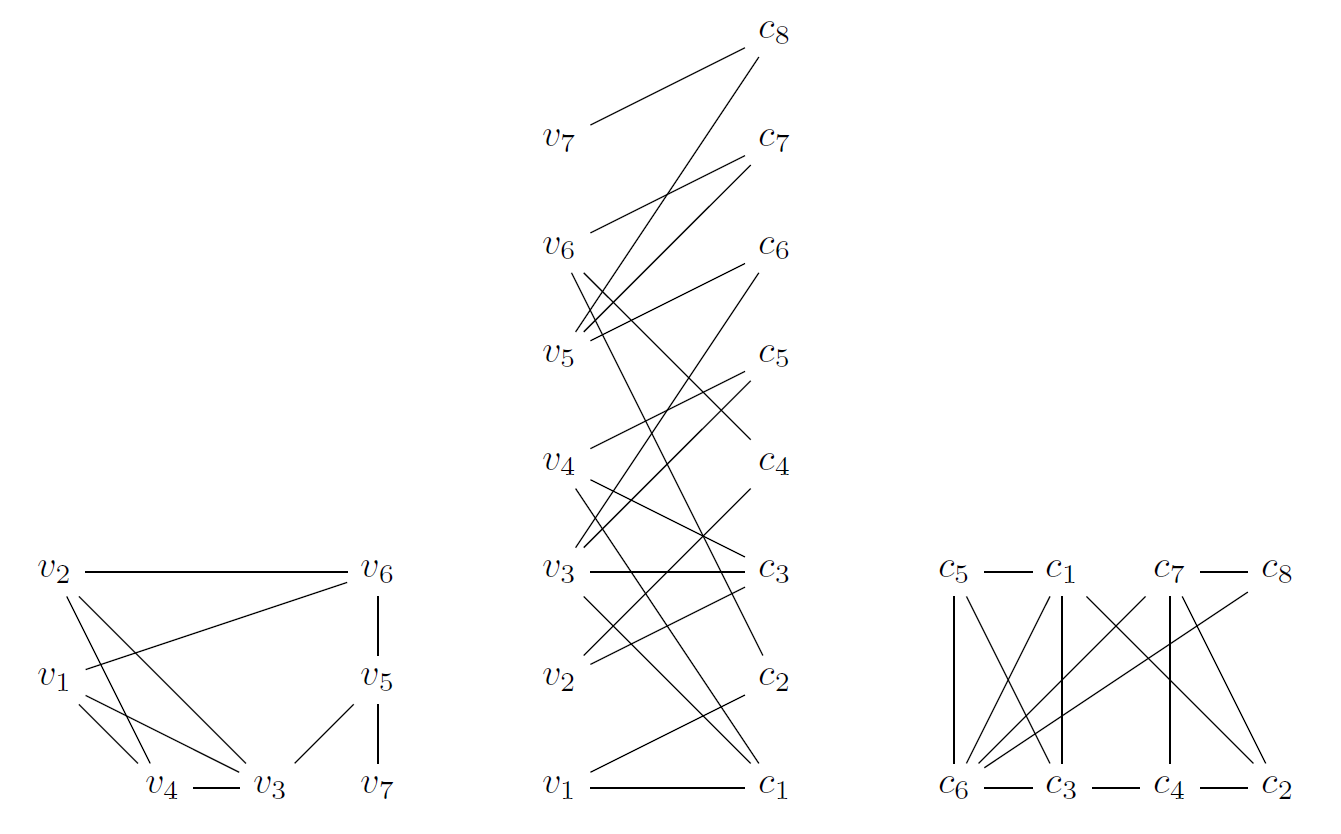
\includegraphics[height=0.5\textheight]{images/DAGraphs.png}
		\caption{The primal (left), incidence (middle) and dual (right) graph}
	\end{figure}
	%\footnotesize{Equivalent CNF}
	%{\tiny $(\neg \text{v1}\lor \neg \text{v3})\land (\neg \text{v1}\lor \text{v6})\land (\text{v1}\lor \neg \text{v4})\land (\neg \text{v2}\lor \neg \text{v5})\land (\neg \text{v2}\lor \text{v6})\land (\neg \text{v3}\lor \neg \text{v4})\land (\neg \text{v3}\lor \text{v5})\land (\neg \text{v5}\lor \neg \text{v6})\land (\text{v5}\lor \text{v7})$}
	
\end{frame}

%%


%\subsection{Example Vertex cover}
%\begin{frame}
%	\frametitle[Vertex Cover]{Example: Vertex-Cover problem}
%
%\end{frame}
%%
%\subsection[Courcelle]{Courcelle's theorem}
%\begin{frame}
%	\frametitle{Courcelle's theorem}
%
%%	\begin{quotation}
%%		Every graph property definable in monadic second-order logic (MSO) is decidable in linear time on graphs of bounded treewidth. \\
%%		\hfill {\small Courcelle, Bruno (1990)}\footnote{Courcelle, Bruno "The monadic second-order logic of graphs. I. Recognizable sets of finite graphs",\\ Information and Computation, 85 (1990) no. 1: 12-75}
%%	\end{quotation}
%
%	\medskip
%	For all $k \in \mathbb{N}$ and MSO-sentences F is the decision problem for a given graph G, whether $G \models F$ is true, in time $2^{p(tw(G))} \cdot |G|$ with a polynom p decidable.
%	\medskip
%	\begin{itemize}
%
%		\item \emph{drawback:} still expensive ($2^{p(tw G)}$, $2^{2^{(\#Q)}}$, large constants) \smallskip 
%		\item usage:
%
%	\end{itemize}
%	\begin{figure}
%		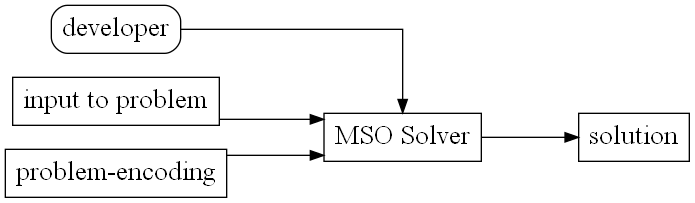
\includegraphics[height=0.2\textheight]{images/UsageCourcelle.gv.png}
%		\caption{Implementation of the theorem}
%	\end{figure}
%\end{frame}


%%%%%%%%%%%%%%%%%%%%%%%
\section{Implementations}

\subsection{gpusat2}
\begin{frame}
	\frametitle{gpusat2 - Solving \#SAT on GPU}
%	=> Dynamic programming Grafiken / Verlaufsschema Kurz erkl�ren -> Beweise dazu sind aufw�ndig und recht spezialisiert / 
	
	%Architecture of our DP-based solver for parallel execution. Yellow colored
	%boxes indicate tasks that are required as initial step for the DP-run or to nally read the
	%model count from the computed results. The parts framed by a dashed box illustrate the
	%DP-part. Boxes colored in red indicate computations that run on the CPU. Boxes colored
	%in blue indicate computations that are executed on the GPU (with waiting CPU).
	\begin{figure}
		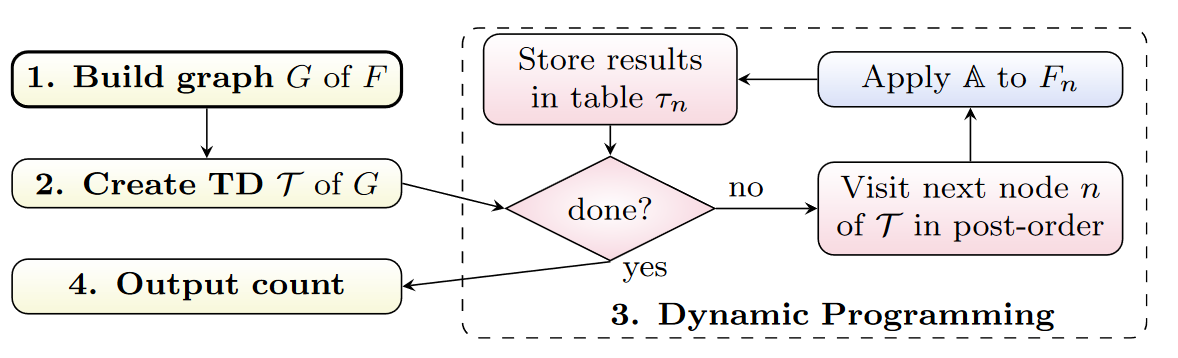
\includegraphics[height=0.3\textheight]{images/DPAlgo31.png}
	\end{figure}
	\medskip
	\begin{minipage}{0.49\textwidth}
		\begin{itemize}
			
			\item Customized tree decompositions
			\item Adapted memory-management
			\item Improved precision handling 
		\end{itemize}
	\end{minipage}
	
\footnotetext{Images: Markus Zisser. \textit{Solving the \#SAT problem on the GPU with dynamic programming and OpenCL}. Technische Universit\"at Wien, 2018.}

%	\begin{minipage}{0.49\textwidth}
%		%Runtime for the top 5 sequential and all parallel solvers over all the #Sat
%		%instances with pmc preprocessor. The x-axis refers to the number of instances and the
%		%y-axis depicts the runtime sorted in ascending order for each solver individually.
%		\begin{figure}
%			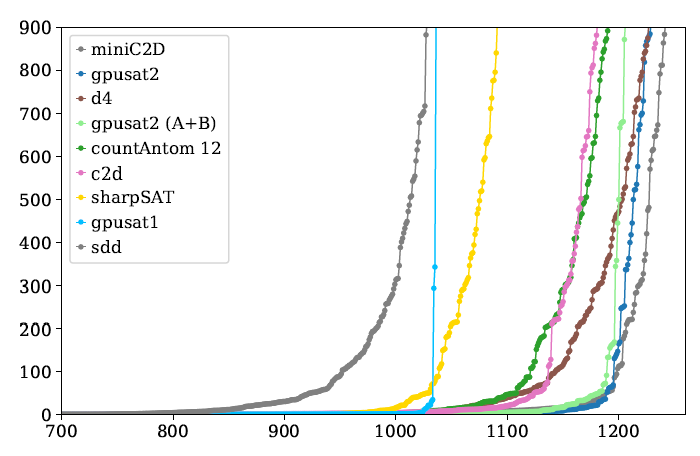
\includegraphics[width=\linewidth]{images/gpusat2Runtime.png}
%		\end{figure}
%	\end{minipage}


\end{frame}
%%
\subsection{dpdb}
\begin{frame}
	\frametitle{dpdb}
%	{\color{blue}Using databases for intermediate results} \medskip\\
	
	Database templates in Python\\
	
	Generating SQL queries	
	


	
	%The idea of dpdb is to use database
	%management systems (DBMS) for table manipulation, which makes it (1) easy
	%and elegant to perform rapid prototyping for problems, and (2) allows to leverage
	%from decades of database theory and database system tuning. It turned out that
	%all the cases that occur in dynamic programming can be handled quite elegantly
	%with plain SQL queries. Our system dpdb can be used for both decision and
	%counting problems, thereby also considering optimization. We see our system
	%particularly well-suited for counting problems, especially, since it was shown
	%that for model counting (#Sat) instances of practical relevance typically have
	%small treewidth [23]. In consequence, we carried out preliminary experiments
	%on publicly available instances for
	\begin{minipage}{0.1\textwidth}
		\hfill
	\end{minipage}
	\begin{minipage}{0.35\textwidth}
			\begin{enumerate}
			\item Create graph representation
			\item Decompose graph
			\item Solve sub-problems
			\item Combine rows
		\end{enumerate}
	
		
	\end{minipage}\hfill
	\begin{minipage}{0.54\textwidth}

		\begin{figure}
			\centering\hfill
			\begin{subfigure}[b]{\textwidth}
				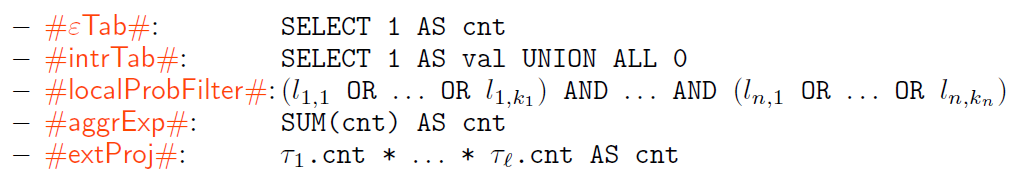
\includegraphics[width=\linewidth]{images/dpdbSSat.png}
				\caption{Problem \#SAT}

			\end{subfigure}\hfill\\
%			\begin{subfigure}[b]{\textwidth}
%				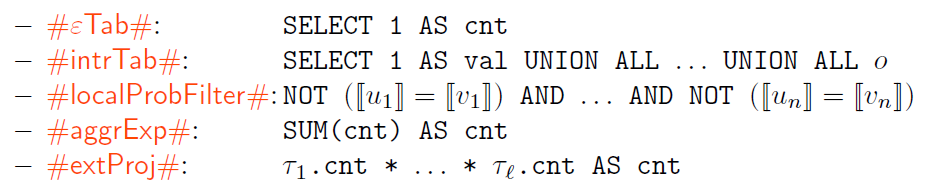
\includegraphics[width=0.8\linewidth]{images/dpdbOCol.png}
%				\caption{Problem }
%			\end{subfigure}\hfill\\
		
			\begin{subfigure}[b]{\textwidth}
				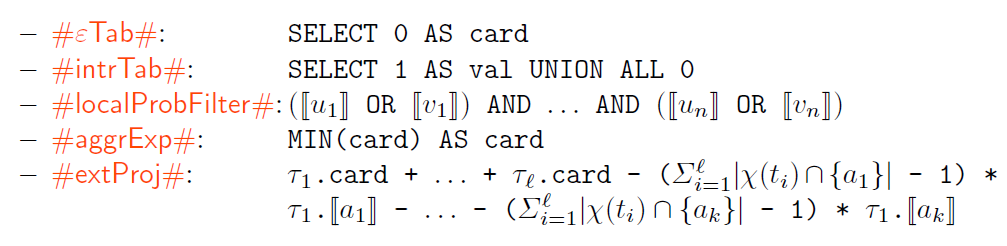
\includegraphics[width=0.8\linewidth]{images/dpdbMinVC.png}
				\caption{Problem MinVC}

			\end{subfigure}
		\end{figure}

	\end{minipage}
\begin{itemize}
	\item SAT and \#SAT
	\item \#o-Coloring
	\item Vertex cover
	\item[] \quad . . .
\end{itemize}
	\footnotetext{``Exploiting Database Management Systems and Treewidth for Counting",\\
		Johannes Fichte et al. doi:	10.1007/978-3-030-39197-3\_10.}
	
\end{frame}


%%%%%%%%%%%%%%%%%%%%%%%
\section{Implementation}
\begin{frame}
	\frametitle{Running tdvisu}
	\medskip

\begin{figure}
	\centering
	
	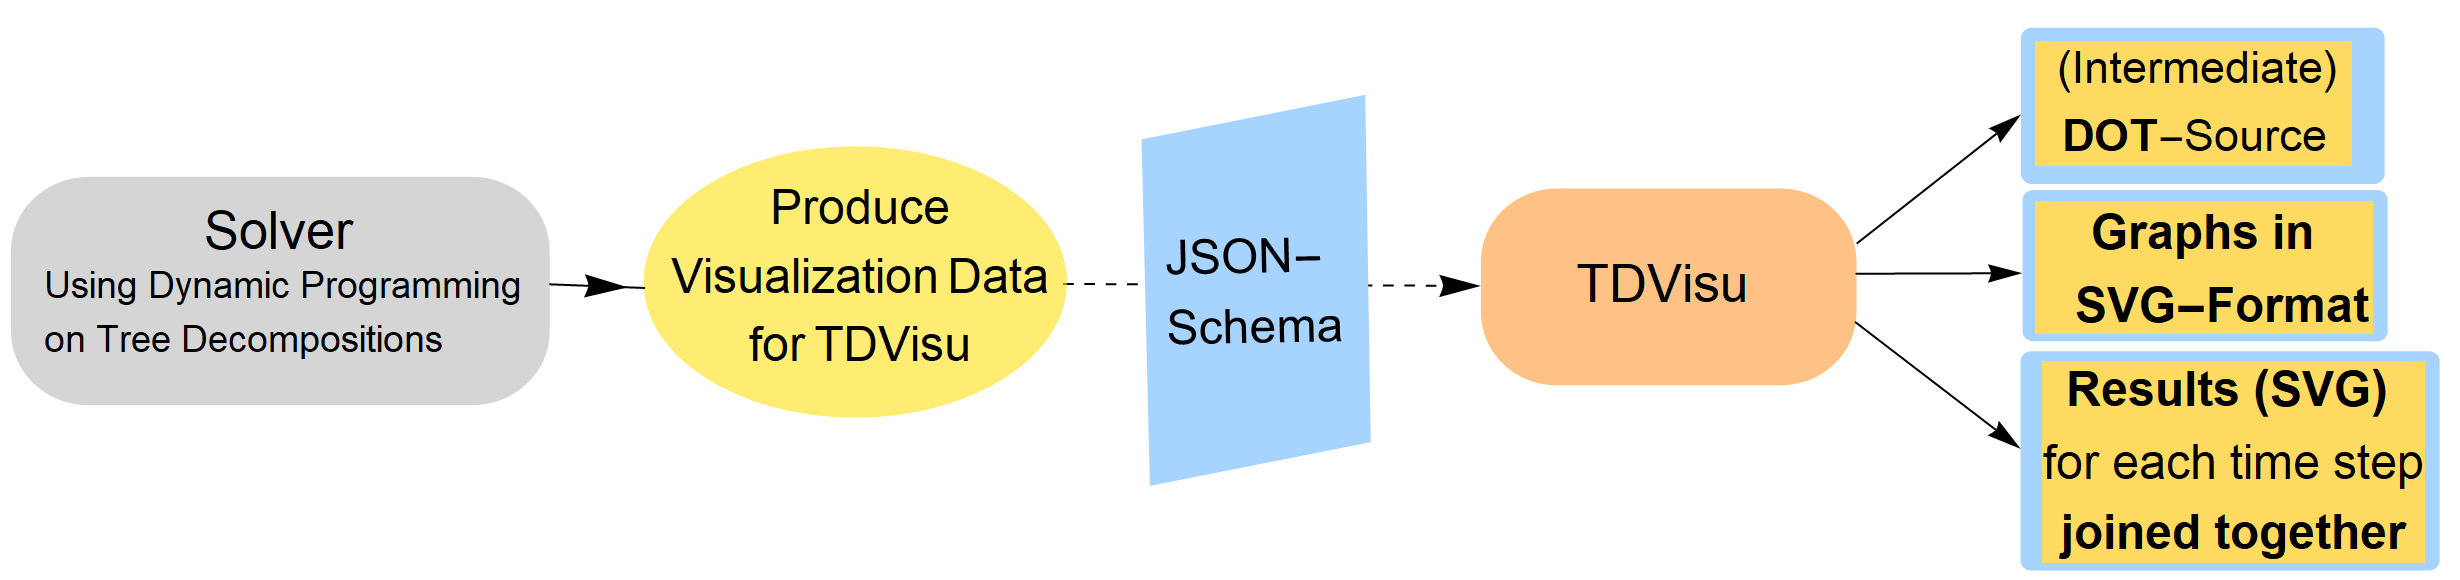
\includegraphics[width=0.95\linewidth]{images/OverviewProgram}
	
	\label{fig:overviewprogram}
\end{figure}
\pause
%	Generisches Datenformat /Strings
%	Visu
%	=> Anwendungen 
\centering
	{TDVisu producing flexible and further processable formats}
	\pause
\begin{figure}
	\centering
	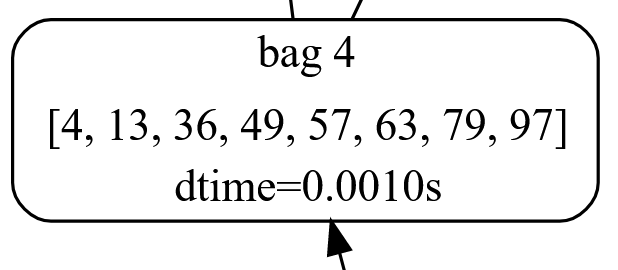
\includegraphics[height=0.25\textheight]{images/Bag4}
	\pause
	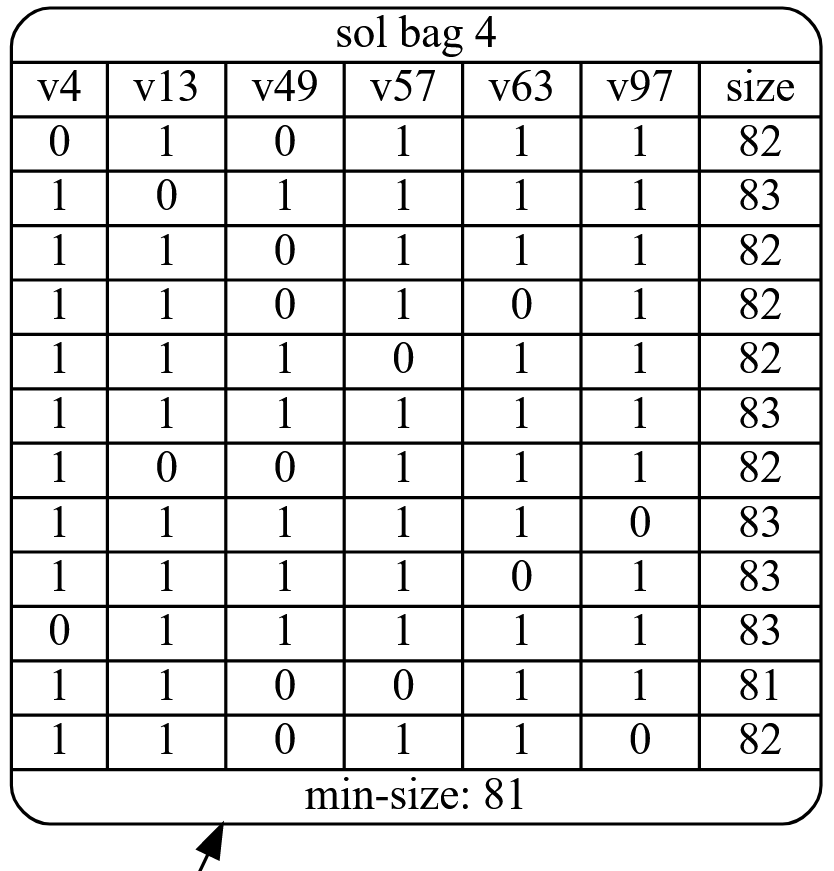
\includegraphics[height=0.45\textheight]{images/SolutionBag4.png}
	\label{fig:bag4}
\end{figure}


		
	
\end{frame}

\begin{frame}
	\frametitle{Challenge2}
	\medskip
	
	 - Wie robust ist die Datenverarbeitung in der Visu
		Restrictions in strings for ids
	 - Was Gedanken bei der Visu waren
	
	
	
	
	
\end{frame}


%%%%%%%%%%%%%%%%%%%%%%%
\section{Visualizing defects}
\begin{frame}
	\frametitle{Visualization in Action}
	\centering
	MinVC example size 90 (expected 82)
	%	show graph of result.
	% 	it is noticeable that neighboring nodes do not contain common nodes.
	
\end{frame}
\begin{frame}
	\frametitle{Visualization in Action}
	\centering
%	MinVC example size 90 (expected 82)
%	show graph of result.
% 	it is noticeable that neighboring nodes do not contain common nodes.
	\begin{enumerate}
		\item Inspect visualization
		\pause
		\item Verify findings in solver (in this case dpdb)
		\pause
		\begin{figure}
			\centering
			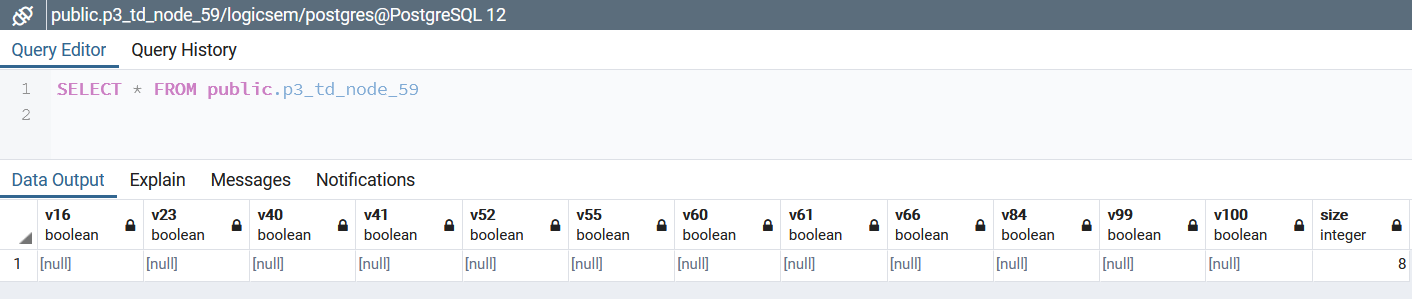
\includegraphics[height=0.2\textheight]{images/Found bag 59 in stars100 with seed0.png}
			\label{fig:faulttdstars}
		\end{figure}
	\pause
		\item Cross reference with standalone tree-decomposition
		\pause
		\begin{figure}
			\centering
			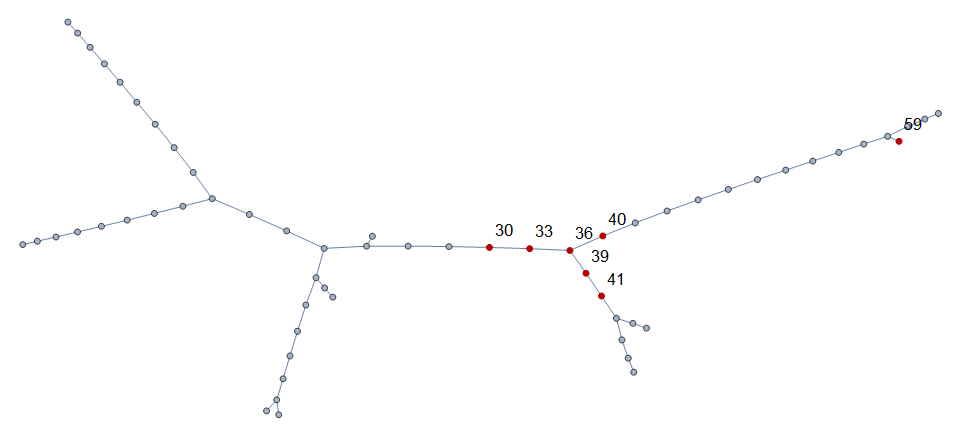
\includegraphics[width=0.5\linewidth]{images/stars100var99}
			\label{fig:stars100var99}
		\end{figure}
	\pause
		\item Fix the root cause
	\end{enumerate}
	

\end{frame}

%%%%%%%%%%%%%%%%%%%%%%%
\section{Related Work}
\begin{frame}
	\frametitle{Related Work on the Algorithms}
%	Related Work Schluss / Wiss Arbeiten 
	\begin{itemize}
		\item Fichte, Johannes \& Hecher, Markus \& Morak, Michael \& Woltran, Stefan. (2018). Exploiting Treewidth for Projected Model Counting and Its Limits. 10.1007/978-3-319-94144-8\_11. 
		\smallskip
		\item Hecher, Markus. (2020). Treewidth-aware Reductions of Normal ASP to SAT - Is Normal ASP Harder than SAT after All?. 485-495. 10.24963/kr.2020/49. 
		
		\medskip
		\item Hecher M., Thier P., Woltran S. (2020)\\
		 Taming High Treewidth with Abstraction, Nested Dynamic Programming, and Database Technology. In: Pulina L., Seidl M. (eds) Theory and Applications of Satisfiability Testing - SAT 2020. SAT 2020. Lecture Notes in Computer Science, vol 12178. Springer, Cham. https://doi.org/10.1007/978-3-030-51825-7\_25
		
	\end{itemize}

\end{frame}
\begin{frame}
	\frametitle{Related Work on Visualizations}
	%	Related Work Schluss / Wiss Arbeiten 
	\begin{itemize}
		\item Marie-Christin Harre, Jan Jelschen, and Andreas Winter. ``ELVIZ: A querybased	approach to model visualization". In: Lecture Notes in Informatics
		(LNI), Proceedings - Series of the Gesellschaft fur Informatik (GI) (Jan.
		2014), pp. 105{120.
		\smallskip
		\item Stephan Diehl. Software Visualization. Visualizing the Structure, Behaviour,
		and Evolution of Software. English. Springer, 2007. 199 pp. isbn: 978-3540465041.
			\medskip
		\item Jason Daida et al. ``Visualizing Tree Structures in Genetic Programming".
		In: Genetic Programming and Evolvable Machines 6 (Mar. 2005). doi: 10.
		1007/s10710-005-7621-2.
		
	\end{itemize}
	
\end{frame}

%%%%%%%%%%%%%%%%%%%%%%%
\section{Other Visualization}

\subsection{Software}
\begin{frame}
	
	
	%	Gephi is a tool for data analysts and scientists keen to explore and understand graphs. Like Photoshop? but for graph data, the user interacts with the representation, manipulate the structures, shapes and colors to reveal hidden patterns.
	
	\begin{figure}
		
\includegraphics[width=0.25\linewidth]{images/gephi.png} \qquad
		
\includegraphics[width=0.25\linewidth]{images/tulip.png} \qquad
		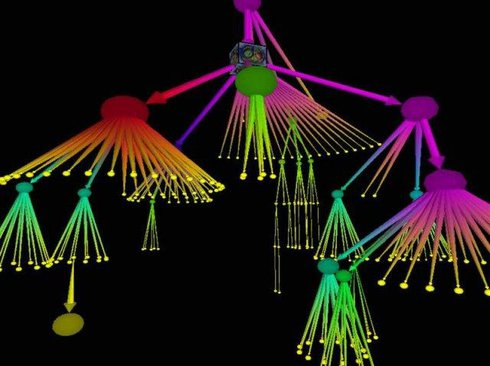
\includegraphics[width=0.15\linewidth]{images/tulip_sample.jpeg}
		\caption*{Gephi.org\footnote{https://gephi.org/ - Tool for data analysts and scientists keen to explore and understand graphs.}
			Tulip  \footnote{tulip.labri.fr/TulipDrupal/ - Better Visualization Through Research.}}
		\label{fig:tulip}
	\end{figure}
	
	
	%	Written in C++ the framework enables the development of algorithms, visual encodings, interaction techniques, data models, and domain-specific visualizations. One of the goal of Tulip is to facilitates the reuse of components and allows the developers to focus on programming their application. This development pipeline makes the framework efficient for research prototyping as well as the development of end-user applications.
	
	\begin{figure}
		
		
\includegraphics[width=0.1\linewidth]{images/visjs_logo.png} \qquad  \qquad
		
\includegraphics[width=0.1\linewidth]{images/sigmajs.png} \qquad
		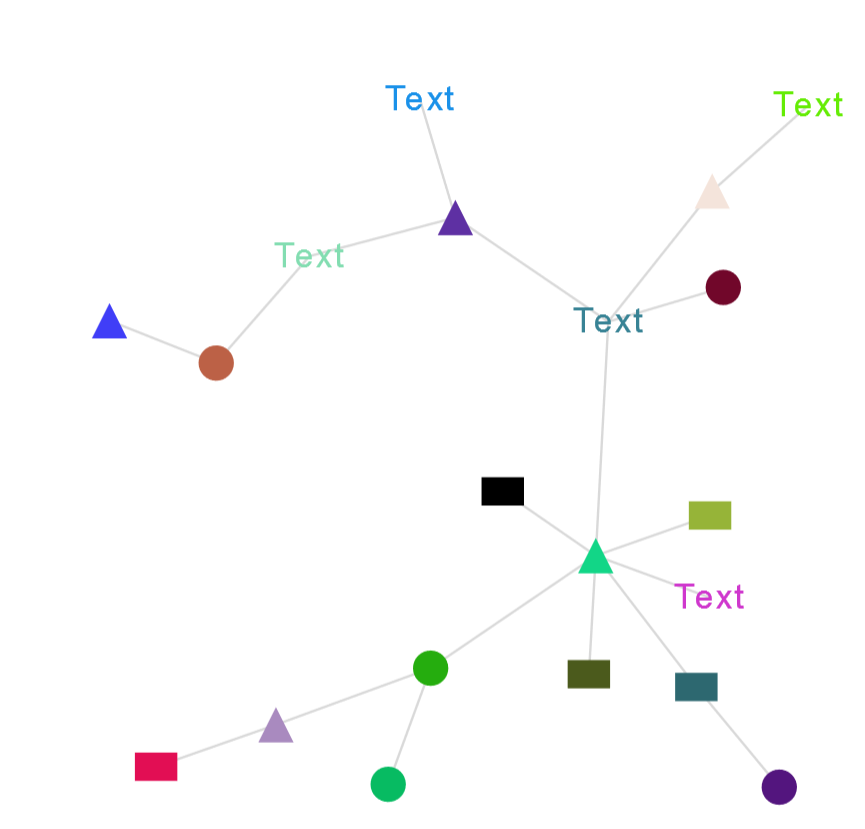
\includegraphics[width=0.15\linewidth]{images/force-graph.png}
		\caption*{ \qquad \qquad \qquad\footnote{https://neo4j.com/developer/tools-graph-visualization/} Vis.js \qquad  \qquad \qquad Sigma.js   \qquad
			vasturiano/3d-force-graph \footnote{https://github.com/vasturiano/3d-force-graph}}
		\label{fig:jsengines}
	\end{figure}
	
	
	%Neovis.js Popoto.js Vis.js Sigma.js ...
	%
	%Commercially licensed:
	%https://www.kineviz.com/graphxr/ 
	%
	%Dynamic Data Modeling, Time Series, Discover correlations, trends, and clusters.
	%%GraphXR is a start-to-finish web-based visualization platform for interactive analytics. For technical users, it?s a highly flexible and extensible environment for conducting ad hoc analysis. For business users, it?s an intuitive tool for code-free investigation and insight.
	%
	%https://github.com/vasturiano/3d-force-graph
	%%3-dimensional representation of a force-directed iterative layout, using 3d-force-graph. This component uses ThreeJS/WebGL for rendering and either d3-force-3d or ngraph for the 3D physics engine.
	%
	%%With this open source library, there are a couple of different components for handling the physics behind three dimensions and for actually rendering the visualization. It uses an iterative approach for rendering in 3D and creates stunning, interactive visualizations. The tool includes features for customizing styles of nodes and relationships, as well as container layouts, rendering controls, configuring simulation, and user interaction. The data structure required is similar to previous tools we have seen, with collections for nodes and relationships. 3d-force-graph also offers functionality for visualizations to use with virtual reality.
	%
	%``ELVIZ: A query-based approach to model visualization" 
	%%about an approach to visualization, generic regarding both the source model, and the kind and content of the visualization.
	%%Marie-Christin Harre, Jan Jelschen, and Andreas Winter. ELVIZ: A querybased
	%%approach to model visualization". In: Lecture Notes in Informatics
	%%(LNI), Proceedings - Series of the Gesellschaft fur Informatik (GI) (Jan.
	%%2014), pp. 105--120.
	
%	Briefly looked up different formats and graph software. 
	With the diverse / large node labels and special layout \\
	the creation of a lightweight and customizable exchange format \\
	took precedence over the integration into special layout software.
\end{frame}

%\subsection{Handcrafted}


%%%%%%%%%%%%%%%%%%%%%%%
\section{Outlook}
\begin{frame}
	\frametitle{Outlook}

%$\rightarrow$ Automatic methods are often more complex than expected. 
	\begin{center}
		\Large Static $\rightarrow$ Dynamic
	\end{center}
	
	\bigskip
	
		Interesting Questions :
		\medskip
	\begin{itemize}
%		for relevant problems the static graph visualization will become to complicated.
%		https://data-science-blog.com/blog/2015/07/20/3d-visualisierung-von-graphen/
		%With particularly extensive and at the same time diverse graphs, a visualization in three or four dimensions (x-, y-, z-dimensions + time t) is not only nicer to look at, but can also be very helpful in gaining an understanding (e.g. via graph clusters).
		\item Utilizing graph databases for visualization and queries for debugging
		\item Enrich the visualization with debugging info for each node
		\item Cross reference the creation of rows in parent nodes
		\item For more advanced debugging tasks you may also need to revise the approach
	\end{itemize}
	
		
		
\end{frame}

%%%%%%%%%%%%%%%%%%%%%%%
\section{Final slide}
\begin{frame}
	\frametitle{Final slide}
%		This thesis created tdvisu as a tool that 
%		\begin{itemize}
%			\item integrates into existing implementations
%			\item statically exports data from runs
%			\item compiles simple DOT files and SVG graphics
%		\end{itemize}
%	\bigskip		
%
%	For further research it provides
%	\begin{itemize}
%		\item starting point for more complex investigations of 
%		\begin{itemize}
%			\item bug spotting
%			\item and fixing by using visualizations
%		\end{itemize} 
%		
%	\end{itemize}
	
%	 into implementations of dynamic programming on tree decompositions 

%	I would like to thank you for your attention.
\end{frame}
%%%%%%%%%%%%%%%%%%%%%%%
\section{BIBLIOGRAPHY}
\begin{frame}
	\frametitle{Bibliography}
	\medskip
	See the citations in the thesis.
\end{frame}
%%%%%%%%%%%%%%%%%%%%%%%

\begin{frame}
	\frametitle{MinVC for example graph}
	\begin{figure}
		\begin{tabular}{c|c}
			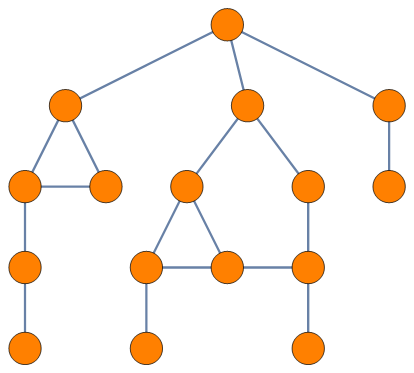
\includegraphics[width=0.45\linewidth]{images/threeGraph1.png} &
		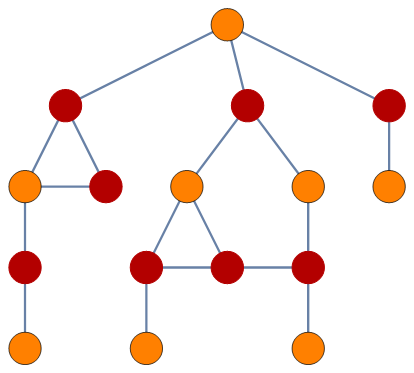
\includegraphics[width=0.45\linewidth]{images/threeGraphOptimal.png}\\
		
		\end{tabular}
	
	\end{figure}
\end{frame}
\begin{frame}
	\frametitle{Visualization}
	\framesubtitle{Manually for one run}
	\begin{figure}
		\centering
		
		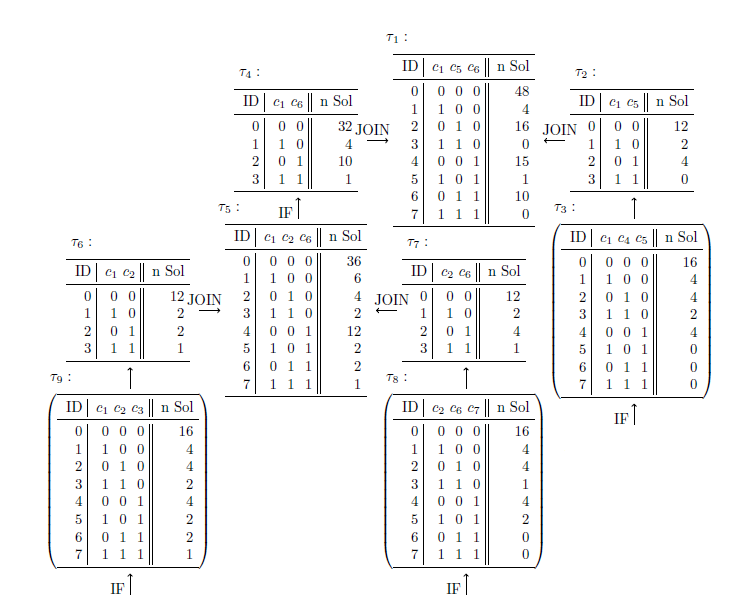
\includegraphics[width=0.55\linewidth]{images/DualDA43.png}		
		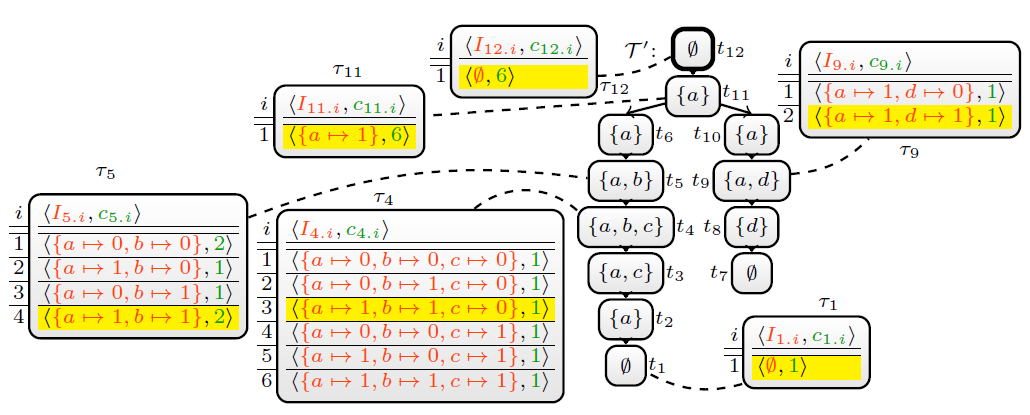
\includegraphics[width=0.44\linewidth]{images/dpdbVisuSat.png}
		
		\caption*{\footnotetext{``Exploiting Database Management Systems and Treewidth for Counting",\\
				Johannes Fichte et al. doi:	10.1007/978-3-030-39197-3\_10.}
			\footnotetext{``Solving \#SAT on the GPU with Dynamic Programming and OpenCL",\\
				Diploma Markus Zisser 2018 Technische Universit\"at Wien, p.33}
			{}}
		\label{fig:dualda43}
	\end{figure}
	
	
\end{frame}
%\begin{frame}
%	\frametitle{Visualization}
%	\framesubtitle{Manually for dpdb}
%	\begin{figure}
%		\centering
%		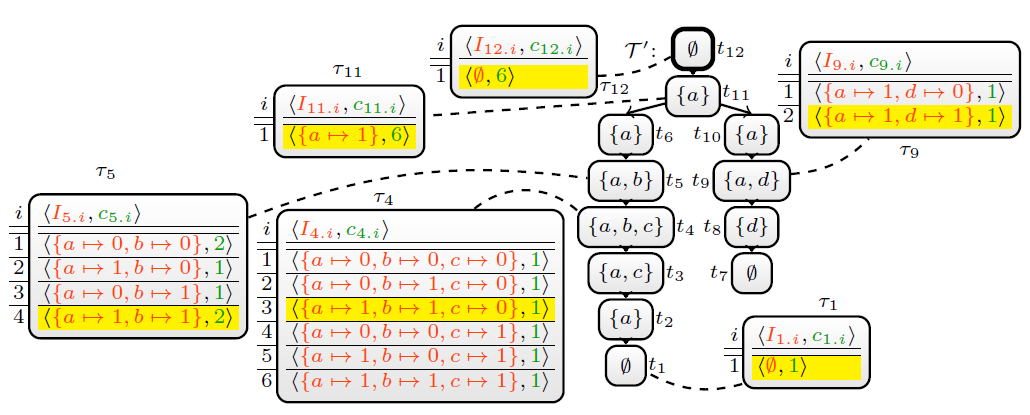
\includegraphics[width=\linewidth]{images/dpdbVisuSat.png}
%		\caption{Handcrafted \#SAT example-run from dpdb\footnote{"Exploiting Database Management Systems and Treewidth for Counting",\\ Fichte, Hecher, Thier, Woltran} }
%		\label{fig:dpdbVisuSat}
%	\end{figure}
%	
%	
%\end{frame}

\begin{frame}
\begin{figure}
	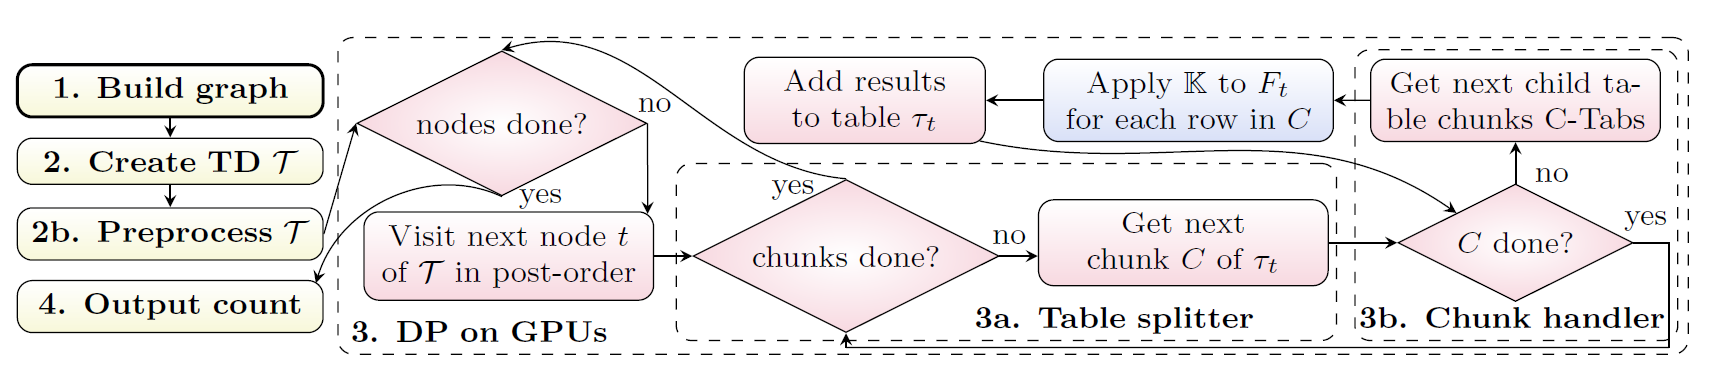
\includegraphics[width=\linewidth]{images/DADPonGPU.png}
\end{figure}
\end{frame}

\begin{frame}
	\medskip
	\frametitle{Benchmark}
	{\color{blue}Performance of all three programs on \#SAT instances:} \medskip\\
	\begin{figure}
		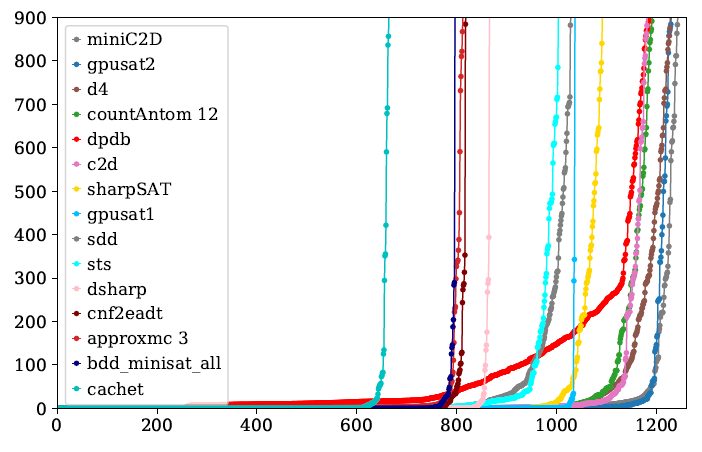
\includegraphics[width=0.8\linewidth]{images/dpdbRuntime.png}
	\end{figure}
\end{frame}

%%%%%%%%%%%%%%%%%%%%%%%%
\bgroup
\setbeamercolor{background canvas}{bg=black}
\begin{frame}[plain]{}
\end{frame}
\egroup

\end{document}